\section{Durchführung}
\subsection{Bestimmung der Zeitkonstante}
Es wird eine Rechteckspannung an den RC-Kreis in Abb.\ref{pic:1} angelegt und
der Spannungsverlauf am Kondensator mithilfe eines Oszilloskopes
graphisch dargestellt. Wenn der Spannungsverlauf der vom Oszilloskop
abgebildet wird von seinem Maximalwert auf 0 abfällt ist dies die Entladekurve und wenn die Spannung wieder von 0 auf den Maximalwert
steigt ist dies die Aufladekurve.
Nun ist ein passender Ausschnitt des Bildschirm zu wählen auf dem eine Auf- und Entladekurve
vorhanden und gut zu erkennen ist. Hier sind die Messwerte an dem Graphen auf dem Osziloskop abzulesen und der Spannungsverlauf
ist digital abzuspeichern.

\begin{figure}[H]
  \centering
  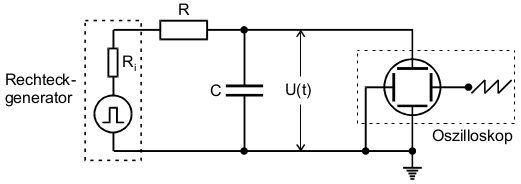
\includegraphics{content/images/pic2.png}
  \caption{Schaltung zur Bestimmung der Zeitkonstante über die Auf- und Entladekurve.}
  \label{pic:2}
\end{figure}

\subsection{Amplitude der Kondensatorspannung}
Für diese Messung wird eine Sinusspannung an den RC-Kreis in Abb.\ref{pic:2} ausgelegt.
Die Amplitude A wird in Abhängigkeit der Frequenz am MilliVoltmeter gemessen, in einem Bereich
Bereich über 3 Zehnerpotenzen der Frequenz. Der Widerstand R soll gemessen werden und untersucht
werden ob $U_0$ frequenzunabhängig ist.

\begin{figure}[H]
  \centering
  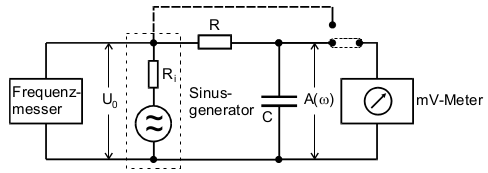
\includegraphics{content/images/pic3.png}
  \caption{Schaltung zur Messung der Zeitkonstante über die Amplitude A($\omega$).}
  \label{pic:3}
\end{figure}


\subsection{Phasenverschiebung in Abhängigkeit von Frequenz}
Zur Messung der Phasenverschiebung zwischen $U_0$ und $U_\text{C}$ verwendet man die Schaltung aus Abb.\ref{pic:3}.
Hierbei wird $U_0$ in Kanal 1 und $U_\text{C}$ in Kanal 2 eingesteckt.
Es wird im Folgenden der Abstand der beiden Schwingungen zwischen den beiden Nullstellen gemessen
und mit der Schwingungsdauer verglichen. Dies wird für die selben Frequenzen wie bei der Amplitudenmessung getan.

\begin{figure}[H]
  \centering
  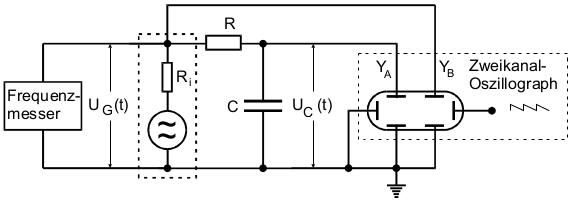
\includegraphics{content/images/pic4.png}
  \caption{Schaltung für Phasenverschiebung.}
  \label{pic:4}
\end{figure}


\subsection{RC-Kreis als Integrator}
Es wird nacheinander eine Rechteck-, Sinus- und dann Dreiecksspannung eingestellt, welche durch den
ersten Kanal des Oszilloskops dargestellt wird. Während die integrierte Spannung durch den zweiten Kanal dargestellt wird.
Anschließend werden die beiden Spannungen passend skaliert und der auf dem Bildschirm zu sehende Verlauf
digital abgespreichert.
